% !TeX root = ../main.tex

\chapter{长寿命粒子模型}

\section{标准模型}


\section{物理背景}
长寿命粒子(Long Lived Particle, LLP)是指在探测器内衰变的时间尺度远大于标准模型粒子的寿命的粒子,它的存在是许多新物理模型的预言。
LLP长寿命的物理机制一般是由于它的衰变被禁戒或是被压低,其中压低可能出于衰变末态粒子的近退简并质量态(nearly-degenerate mass states)或是沟通LLP与末态粒子的相互作用强度微弱。
由于LLP具有较长的寿命、与标准模型粒子仅存在微弱的相互作用,因此它常被认为是暗物质的候选者。

由于LLP能在衰变前行进一定的宏观距离,其衰变产物不会从原始碰撞点(Primary Vertices)产生,而是在远离大多数标准模型粒子产生的初级顶点处形成一个次级顶点(Secondary Vertices),
该顶点也被称为偏离对撞顶点(Displaced Vertices)。
进一步,当LLP的衰变位置在电磁量能器之后时,其衰变产物会在电磁量能器内沉积少量能量,并且在其后的强子量能器内沉积绝大部分能量。
通过定义喷注在两类量能器中沉积的能量比值$$\text{CalRatio}=E_{\text{H}}/E_{\text{EM}}$$
其中$E_{\text{H}}$为强子量能器内沉积的能量、$E_{\text{EM}}$电磁量能器内沉积的能量,可以作为鉴别LLP的衰变的重要参数。\cite{calratio}

尽管目标LLP是在强子量能器中才发生衰变,但我们仍预期在电磁量能器中会有少量的能量沉积,原因有二。
其一是本分析对于在电磁量能器的后端发生衰变的LLP仍然敏感,该情况同样会导致较高的 CalRatio 值。
其二是由于一些与信号无关的现象可能会导致在电磁量能器中沉积能量。

\begin{figure}[ht]
    \centering
    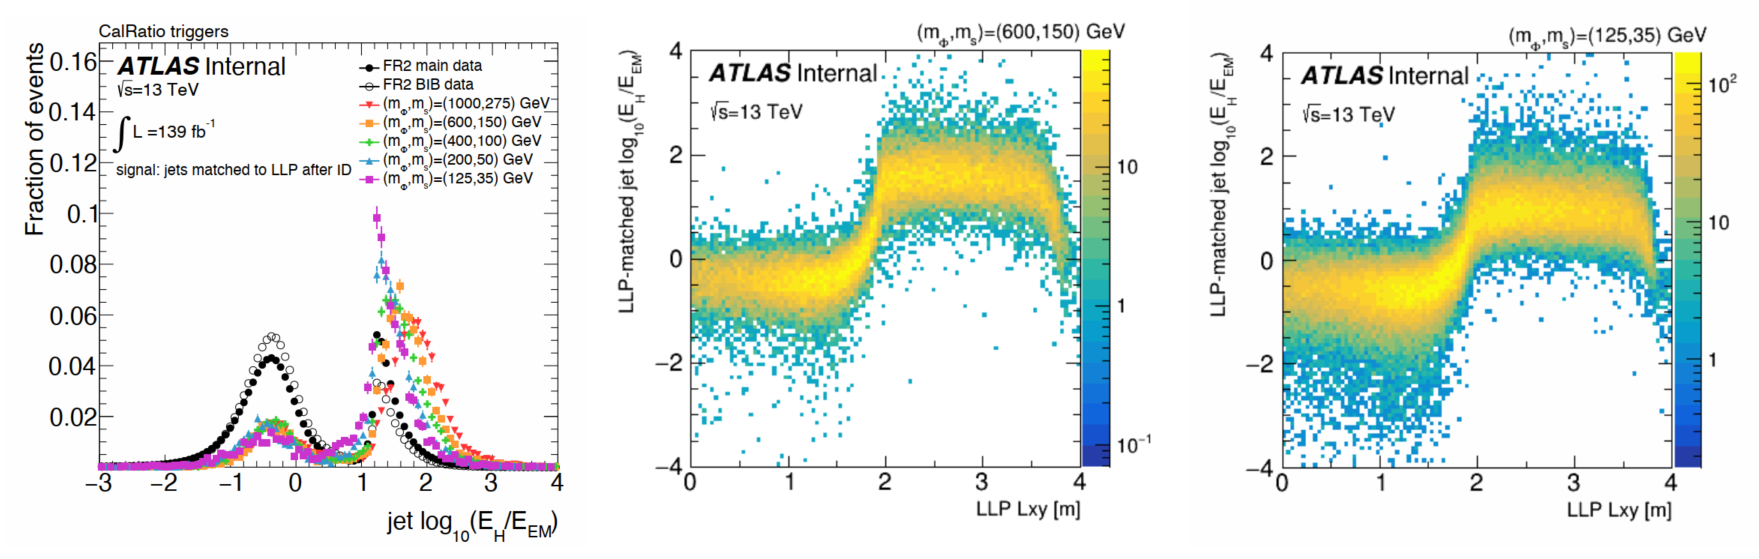
\includegraphics[width=\textwidth]{CalRatioDistribution.png}
    \caption{CalRatio分布图}
    \label{fig:CalRatioDistribution}
    \figurenote{
        左图:探测器数据、BIB数据与五个不同的信号数据的$\log_{10}\text{CalRatio}$分布图,
        中图、右图:在两个不同的信号数据的$\log_{10}\text{CalRatio}$关于$L_{xy}$的分布图。
    }
\end{figure}

从\autoref{fig:CalRatioDistribution} 的左图可以看出,LLP的信号数据在$\log_{10}\text{CalRatio}$分布上与背景数据有明显的区别,
在$-1.5<\log_{10}\text{CalRatio}<0.5$的区间背景数据分布比例高而信号数据分布比例低,
而在$1<\log_{10}\text{CalRatio}<2.5$的区域背景数据分布比例低而信号数据分布比例高。
\autoref{fig:CalRatioDistribution} 的中图、右图则是两类LLP在不同的$x$--$y$平面衰变位置$L_{xy}$下$\log_{10}\text{CalRatio}$的分布,
其中筒部的电磁量能器位于$\SI{1.5}{m} < L_{xy} < \SI{2}{m}$处、强子量能器位于$\SI{2}{m} < L_{xy} < \SI{4}{m}$处,
所以在$L_{xy} > \SI{2}{m}$时LLP的衰变产物会显著减少在电磁量能器内沉积的能量,因而能观察到$\log_{10}\text{CalRatio}$显著增加。

\begin{figure}[ht]
    \centering
    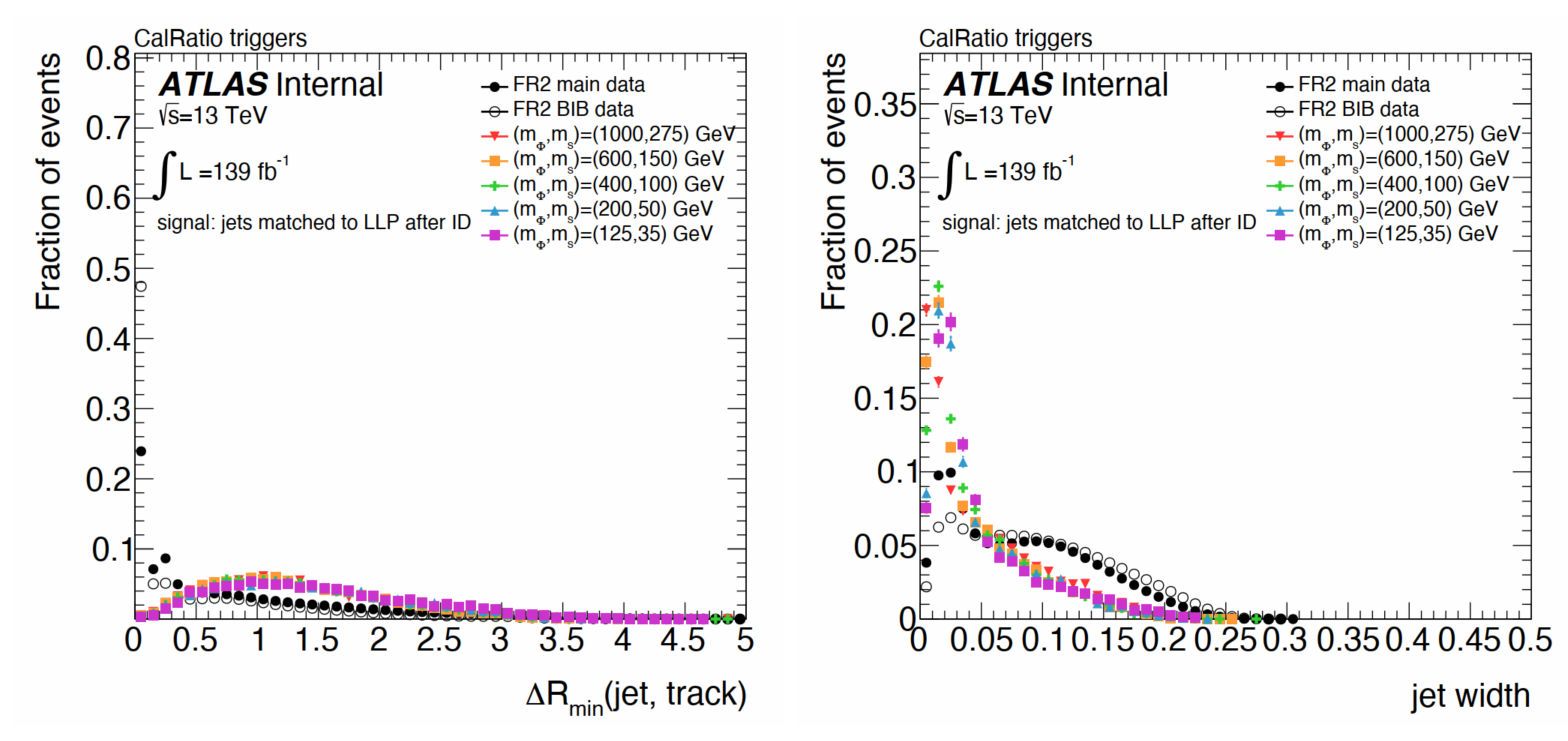
\includegraphics[width=0.85\textwidth]{DR_jet_width.png}
    \caption{$\Delta R_{\min}$与喷注宽度的分布图}
    \label{fig:DR_jet_width}
    \figurenote{
        左图:喷注中$p_T>\SI{2}{GeV}$的径迹距离喷注轴线方向的最小角距离的分布图,角距离$\Delta R = \sqrt{(\Delta \phi)^2+(\Delta \eta)^2}$;
        右图:喷注宽度的分布图,喷注宽度定义为以$p_T$加权的次级粒子与喷注轴线的角距离。
    }
\end{figure}

由于LLP的衰变发生在量能器而非初级顶点,喷注中的粒子能够在探测器中扩散的时间与距离减少,导致喷注宽度变小。
从\autoref{fig:DR_jet_width} 可以看出相较于LLP产生的喷注,标准模型的喷注可能有部分更靠近轴线方向的次级粒子,
但考虑所有粒子角距离的贡献后,它的喷注宽度是更宽的。

综上所述,我们可以通过物理量诸如CalRatio与喷注宽度来区分LLP产生的喷注与标准模型的喷注。
该思想将被运用到数据获取的触发与后续的分析中。


\section{具体模型}

\subsection{Hidden Sector 模型}

\subsection{超对称模型}
标准模型为夸克、轻子、规范玻色子被规范群$SU(3)\times SU(2) \times U(1)$控制的可重整理论。
为了解释等级问题(hierarchy problem),也即引力在 \num{e16} 到 \SI{e18}{GeV} 之间的某个能量与其他四种相互作用的统一,
我们需要引入超对称性(supersymmetry)来将费米子与玻色子结合在一起。

超对称模型引入两个左手征超场的$SU(2)$二重态
$$H_1 = \mqty(H_1^0 \\ H_1^-) \qc H_2 = \mqty(H_2^+ \\ H_2^0) $$
来产生$SU(2) \times U(1)$的自发对称破缺并赋予所有夸克、轻子以及$W^\pm$和$Z^0$质量。
同时每个费米子都有一个玻色子伴侣、每个玻色子都有一个费米子伴侣。
\cite{QFT_Weinberg}

为了防止质子在超对称模型中衰变得太快,通常需要引入R宇称并要求它守恒,它定义为
\begin{equation}
    R = (-1)^{3(B-L)+2S}
\end{equation}
其中$B$为重子数、$L$为轻子数、$S$为自旋量子数。
对于所有的标准模型粒子,$R=1$;对于所有的超对称粒子,$R=-1$。
\cite{SUSY_ATLAS}

当R宇称守恒时,最轻的超对称粒子(lightest supersymmetry particle, LSP)是稳定的,因此LSP是暗物质的优秀候选者。
超对称粒子也有是LLP的候选者。

\subsection{Higgs-portal baryogenesis models}

